\documentclass[12pt]{article}
 
\usepackage[margin=1in]{geometry} 
\usepackage{amsmath,amsthm,amssymb,bm}
\usepackage{graphicx}
%\usepackage{subcaption} % To use subfigures with subcaptions
\usepackage[caption = false]{subfig}
 
\begin{document}
  
\title{Task 2. Mesh Animation}
\author{Garoe Dorta-Perez\\
CM50245: Computer Animation and Games II}
 
\maketitle
 
\section{Introduction}

Generating a realistic morphing between two meshes can be a challenging task.
We present two approaches to produce a intermediate 3D mesh from conforming source and target 3D meshes. 

\section{Linear interpolation}

Linear interpolation is a simple and intuitive approach.
The new position of a vertex $\mathbf{v}_{it} = \left[ v_{ix}, v_{iy}, v_{iz}\right]^T $ in an interval $t = \lbrace 0, \ldots, 1 \rbrace$ is given by

\begin{equation*}
\mathbf{v}_{it} = (1 - t) \mathbf{p}_i + t \mathbf{q}_i \quad i \in \lbrace 1, \ldots, n \rbrace,
\end{equation*}

where $n$ is the number of vertices, $\mathbf{p}_i = \left[ p_x, p_y, p_z\right]^T$ and $\mathbf{q}_i = \left[ q_x, q_y, q_z\right]^T$ are corresponding vertices in the source and target meshes, respectively.
Meshes generated with this method are shown in Figure \ref{fig:linearInterpolation}.

\section{As-rigid-as-possible interpolation}

The previous method produces distorted meshes due to its non-rigid nature.
One way to produce better results is to use transform-based techniques \cite{Alexa2000}.
Let us define an affine transformation from $\mathbf{p}_i$ to $\mathbf{q}_i$ such that

\begin{align*}
A_j \mathbf{p}_i + \mathbf{l}_j = \begin{pmatrix}
 a_{11} & a_{12} & a_{13} \\ 
 a_{21} & a_{22} & a_{23} \\ 
 a_{31} & a_{32}  & a_{33} 
\end{pmatrix} 
\begin{pmatrix}
 p_{ix} \\ 
 p_{iy} \\ 
 p_{iz} 
\end{pmatrix} +
\begin{pmatrix}
 l_x \\ 
 l_y \\ 
 l_z
\end{pmatrix} = \mathbf{q}_i.
\end{align*}

We have a matrix $A_{j}$ and a translation vector $\mathbf{l}_j$ for each triangle.
An extra vertex is added to every triangle, to be able to compute $A_j$, since with the three points in a triangle, we can only built an underconstrained system, with 12 unknowns and 9 equations.
This extra vertex position is calculated as $\mathbf{p}_{new} = \mathbf{c}_{tr} + w\mathbf{n}_{tr}$, where $\mathbf{c}_{tr}$ is the triangle centroid, $w$ is the average triangle edge length and $\mathbf{n}_{tr}$ is the triangle normal. 
In a mesh vertices are shared among different triangles, so we cannot transform each triangle independently with its $A_j$.
Instead let us define $B_{j}$ as the matrix that would transform the vertices in the triangle consistently.
$A_j$ and $B_j$ are related by

\begin{equation*}
E(t) = \sum_{j}^J \left \| A_j(t) - B_j(t) \right \|^2_F,
\end{equation*}

where $\left \| \cdot \right \|_F$ is the matrix Frobenius norm, and the objective is to minimize $E(t)$.
The underlying logic of this minimization is to compute a $B_j$ that is as similar as possible to $A_j$, subject to the vertex constraints.
In order to treat each vertex in the mesh consistently, instead of having $\mathbf{q}_i$ for each triangle, let us consider them into a vertex $\mathbf{v}_i$ in the mesh.
For each triangle, we can stack all its vertices in a matrix such as

\begin{equation*}
\begin{bmatrix} P | I \\ P_e | I_e \end{bmatrix} \begin{bmatrix}  B_{col} \\ \mathbf{l} \end{bmatrix} = 
\begin{pmatrix}
 \mathbf{p}_1^T & \mathbf{0} & \mathbf{0} & 1 & 0 & 0\\ 
 \mathbf{0} & \mathbf{p}_1^T & \mathbf{0} & 0 & 1 & 0\\ 
 \mathbf{0} & \mathbf{0} & \mathbf{p}_1^T & 0 & 0 & 1\\
  \mathbf{p}_2^T & \mathbf{0} & \mathbf{0} & 1 & 0 & 0\\ 
 \mathbf{0} & \mathbf{p}_2^T & \mathbf{0} & 0 & 1 & 0\\ 
 \mathbf{0} & \mathbf{0} & \mathbf{p}_2^T & 0 & 0 & 1\\
  \mathbf{p}_3^T & \mathbf{0} & \mathbf{0} & 1 & 0 & 0\\ 
 \mathbf{0} & \mathbf{p}_3^T & \mathbf{0} & 0 & 1 & 0\\ 
 \mathbf{0} & \mathbf{0} & \mathbf{p}_3^T & 0 & 0 & 1 \\
   \mathbf{p}_e^T & \mathbf{0} & \mathbf{0} & 1 & 0 & 0\\ 
 \mathbf{0} & \mathbf{p}_e^T & \mathbf{0} & 0 & 1 & 0\\ 
 \mathbf{0} & \mathbf{0} & \mathbf{p}_e^T & 0 & 0 & 1
\end{pmatrix}
\begin{pmatrix}
b_{11} \\
b_{12} \\
b_{13} \\
b_{21} \\
b_{22} \\
b_{23} \\
b_{31} \\
b_{32} \\
b_{33} \\
l_{1} \\
l_{2} \\
l_{3}
\end{pmatrix} =
\begin{pmatrix} 
v_{1x} \\
v_{1y} \\
v_{1z} \\
v_{2x} \\
v_{2y} \\
v_{2z} \\
v_{3x} \\
v_{3y} \\
v_{3z} \\
v_{ex} \\
v_{ey} \\
v_{ez}
\end{pmatrix},
\end{equation*}

\begin{equation*}
P^{-1} = 
\begin{pmatrix}
\alpha_1 & 0 & 0 & \delta_1 & 0 & 0 & \lambda_1 & 0 & 0 \\
\alpha_2 & 0 & 0 & \delta_2 & 0 & 0 & \lambda_2 & 0 & 0 \\
\alpha_3 & 0 & 0 & \delta_3 & 0 & 0 & \lambda_3 & 0 & 0 \\
0 & \beta_1 & 0 & 0 & \epsilon_1 & 0 & 0 & \mu_1 & 0 \\
0 & \beta_2 & 0 & 0 & \epsilon_2 & 0 & 0 & \mu_2 & 0 \\
0 & \beta_3 & 0 & 0 & \epsilon_3 & 0 & 0 & \mu_3 & 0 \\
0 & 0 & \gamma_1 & 0 & 0 & \kappa_1 & 0 & 0 & \pi_1 \\
0 & 0 & \gamma_2 & 0 & 0 & \kappa_2 & 0 & 0 & \pi_2  \\
0 & 0 & \gamma_3 & 0 & 0 & \kappa_3 & 0 & 0 & \pi_3
\end{pmatrix},
\end{equation*}

where $\mathbf{p_e}$ is the extra vertex in the source triangle and $\mathbf{v_e}$ is the extra vertex in the target triangle.
The $\mathbf{l}_j$ terms can be ignored as they only represent triangle position in the scene, and we are interested in its shape and rotation.
Extracting the matrices of interest to us, we have $B = P^{-1}V$, so $B$ can be expressed as a linear combination of matrix $V$.
We would have the above system for each triangle in the mesh, with its own $P$ and $B$ matrices.  
Writing explicitly the Frobenius terms in $E(t)$, and using the above expression to substitute each $B$ term for $\mathbf{v}_i$ terms, we get

\begin{align*}
E(t) &= \lbrace a_{11}^2 - 2 a_{11} b_{11} + b_{11}^2 + \cdots +  b_{33}^2 \rbrace_{j = 1} + \ldots + \lbrace \cdots \rbrace_{j = J} \\ 
& = \lbrace a_{11}^2 + a_{12}^2 + \ldots + a_{33}^2 + \alpha_1^2 v_{1x}^2 + \ldots + \pi^2 v_{3z}^2 - 2 a_{11} \alpha_1 v_{1x} \\
& - 2 a_{11} \delta_1 v_{2x} - 2 a_{11} \lambda_1 v_{3x} - \ldots - 2 a_{33} \pi_3 v_{3z} + 2 \alpha_1 v_{1x} \delta_1 v_{2x} \\ 
& + 2 \alpha_1 v_{1x} \lambda_1 v_{3x} + \ldots + 2 \kappa_3 v_{2z} \pi_3 v_{3z} \rbrace_{j = 1} + \ldots + \lbrace \cdots \rbrace_{j = J},
\end{align*}

where we have a $\lbrace \cdots \rbrace_j$ term for each triangle.
If we set the transformation of $\mathbf{v_1}$ to linear interpolation, and defining 
$\mathbf{u}(t)^T = \begin{pmatrix} 1, v_{2x}, v_{2y}, v_{2z}, \ldots, v_{mx}, v_{my}, v_{mz} \end{pmatrix}$, where $m$ is the number of vertices, we can stack the terms in a quadratic matrix form 

\begin{equation*}
E(t) = \mathbf{u}^T  \begin{pmatrix}
c & \mathbf{g}(t)^T \\
\mathbf{g}(t) & H
\end{pmatrix} \mathbf{u},
\end{equation*}

where $c$ are the constant coefficients, $\mathbf{g}$ is a vector with the linear terms and $H$ is matrix with the quadratic and mixed terms.
Note that, since $\mathbf{v}_1$ is known, the terms were it appears become constants or linear in $\mathbf{v}_j$ for $j \neq 1$.
A solution for the system can be found by setting the gradient to zero

\begin{equation*}
H \mathbf{u}(t) = -\mathbf{g}(t) ~ \rightarrow ~ \mathbf{u}(t) = - H ^{-1} \mathbf{g}(t).
\end{equation*}

Since $H$ is independent on $t$, for each iteration only the linear interpolation of $\mathbf{v}_1$ and the new $\mathbf{g}(t)$ have to be computed to solve the system.

\section{Results and conclusions}

Figure \ref{fig:linearInterpolation} shows that, applying a vertex based linear interpolation rescales the interpolated mesh into unnatural positions.
For example, the interpolated horse head in Figure \ref{fig:linearHorse1} is smaller than the original head in the source and target shape.
Applying the as-rigid-as-possible interpolation produces better results because it interpolates the transformation matrices, instead of the vertex positions.

\begin{figure}
\subfloat[Linear interpolation]{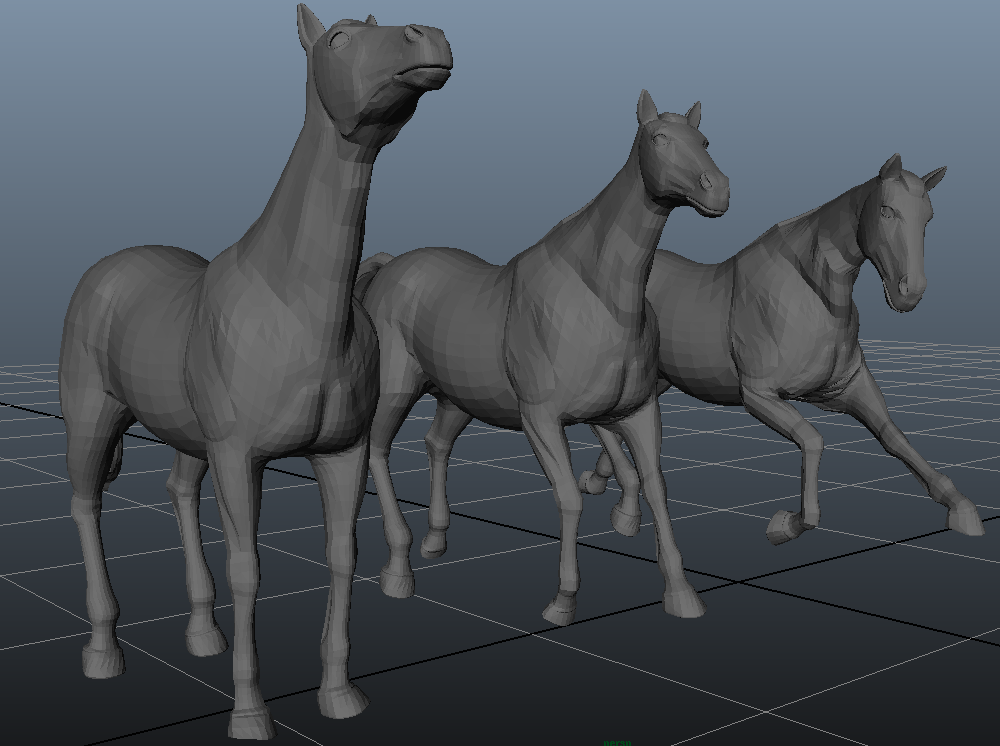
\includegraphics[width = 3in]{images/linearInterpolation2} \label{fig:linearHorse1}}
\thinspace
\subfloat[Linear interpolation]{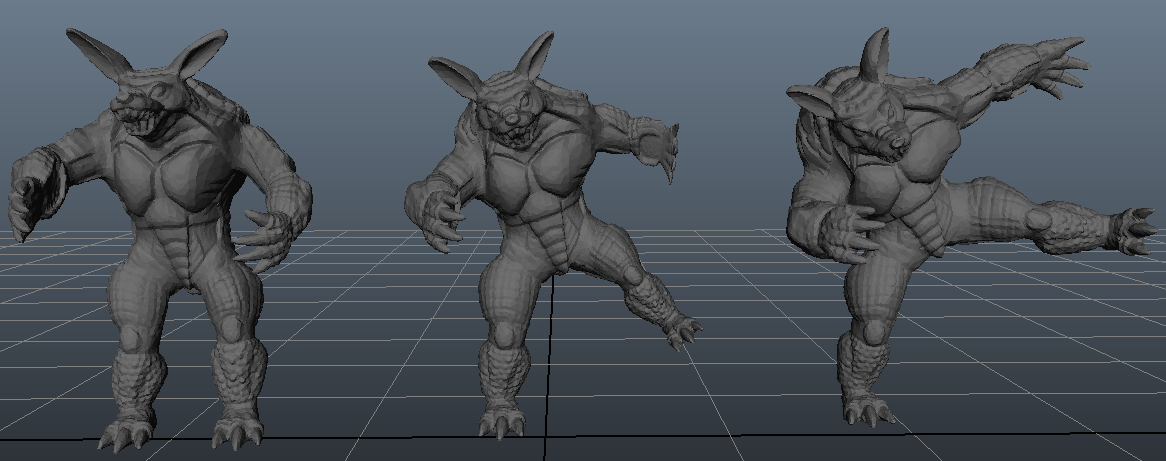
\includegraphics[width = 3.5in]{images/linearArmadillo}} \\
\subfloat[Rigid interpolation]{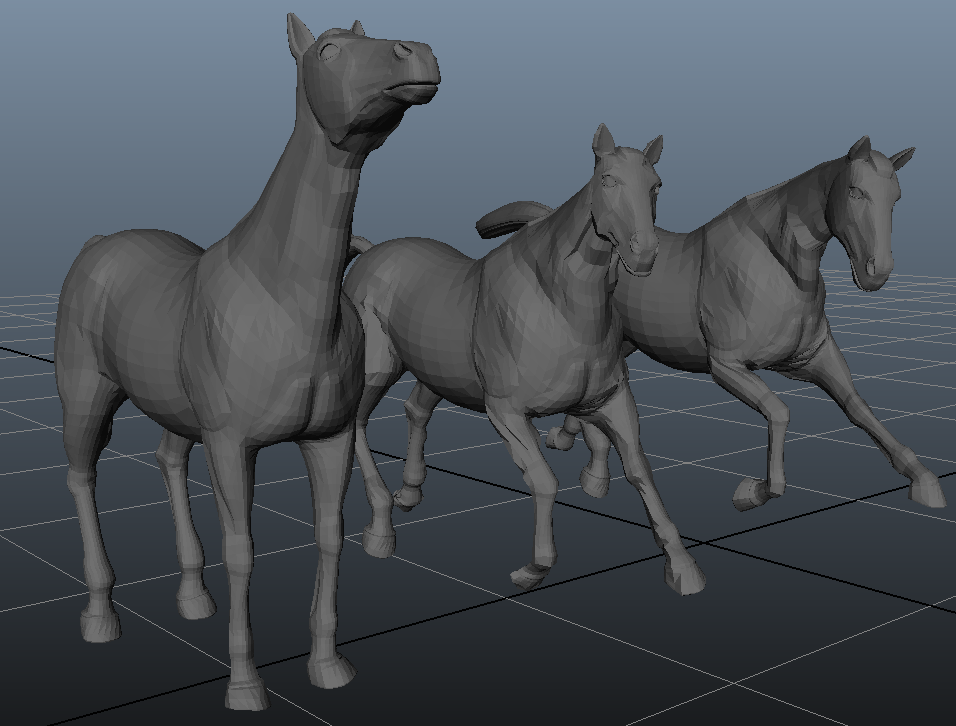
\includegraphics[width = 3in]{images/transformInterpolation2}}
~
\subfloat[Rigid interpolation]{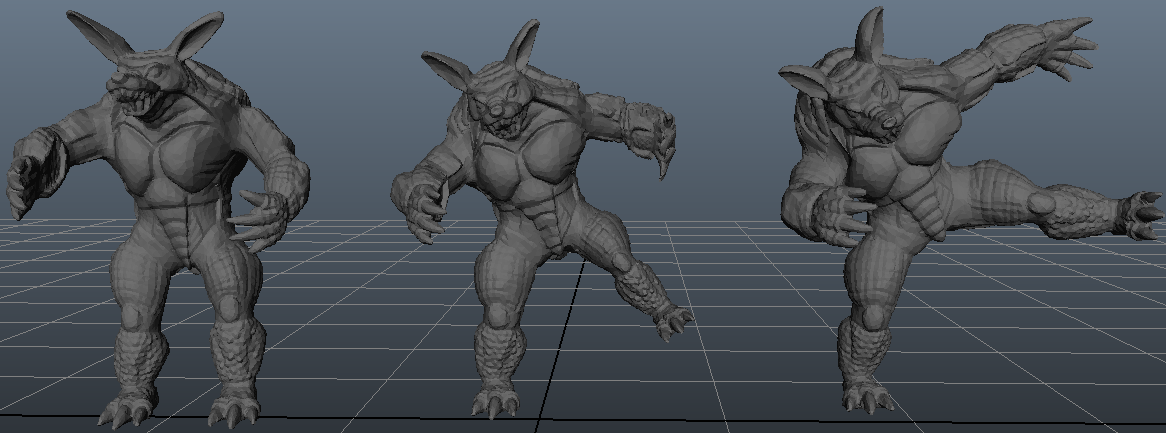
\includegraphics[width = 3.5in]{images/rigidArmadillo}} 
\caption{Horse and armadillo meshes, morphed mesh is in the middle.}
\label{fig:linearInterpolation}
\end{figure}

\bibliographystyle{plain}
\bibliography{t2_meshAnim}

\end{document}

